This chapter briefly describes a discrete-time dynamical system and what it means to exhibit chaos. We refer to \cite{devaney2018introduction, de2013elements} for more details. 

At its most elementary level, a dynamical system is just something that evolves deterministically through time. In the context of this project, deterministic refers to the fact that a system evolves according to specified rules rather than based on random events. 
Dynamical systems arise in a variety of situations. A continuous-time dynamical system describes the states for all values of the time. Specifically, if the motion of a pendulum in which the quantities such as the angular position and angular momentum are known at all times, then it is a continuous-time dynamical system. The equations of the dynamical system can take the form of one or more ordinary differential equations that determine the relevant quantities at any future time if we know the initial location and momentum. 
In ecology, discrete-time dynamical systems are widely used to model population growth. The model in this case is a function calculating the following generation's population given the population of the previous generation. If we know the starting population, we may once again calculate the population at any time in the future. 

Formally, a function $T: U \to U$, where $U$ is some set is  a \emph{discrete-time dynamical system} and its iterates $\{u,Tu,T^2u,\ldots\}$, where $T^n$ denotes the $n$-fold composition of $T$ with itself, describe the evolution of an initial condition $u\in U$ (Note that we frequently drop the brackets and denote $T(u)$ by $Tu$ so as to simplify notations).  





Continuous-time dynamical systems modelled using ordinary differential equations can give rise to discrete-time dynamical systems. To see this, consider a differential equation $\dot{x} = f(x)$, $f: \mathbb{R}^n \to \mathbb{R}^n$, $n\in\mathbb{N}$ given to have a unique solution passing through 
each point $x\in\mathbb{R}^{n}$, call it $x(t)$ where $x(0)=x_0$. 

\begin{Definition}
  [\bf Flow of an Equation] \label{Dfn_Flow}\rm
  The flow of the equation  $\dot{x} = f(x)$  is defined to be a mapping $\varphi: \mathbb{R}^n \times \mathbb{R} \to \mathbb{R}$ where $\varphi(x_0,t)= x(t)$ for the solution $x(t)$ with $x(0)=x_0$ 
\end{Definition}

By fixing $t=K \in (0,\infty)$, we can define the \emph{time-$K$ map} as  $T(x):= \varphi(x_0,K)$, and it is easily verified that $T\circ T(x_0) = \varphi(x_0,2K)$. In general the $m^{\mbox{th}}$ iterate of $x_0$ under $T$ would be the value of the solution of the ODE evaluated at time $mK$ with the initial condition $x_0$, i.e. $\varphi(x_0, mK)$. 
Thus ordinary differential equations give rise to a discrete-time dynamical system by sampling the value of the solution $x(t)$ at time intervals $K$ units apart. 


A numerical discretization of a differential equation can also give rise to a discrete-time dynamical system. For instance, Euler's method approximates $\dot{x}(t)$ by $(x(t+h)-x(t))/h$; if $h$ is fixed throughout, the solution of a differential equation $\dot{x}=f(x)$ 
can be approximated at the time instant $t+(m+1)h$ by iterating the equation 
\begin{equation}
  x(t+(m+1)h) = x(t+mh) + h f(x(t+mh))
\end{equation}

Adopting more succinct notation by replacing $x(t+mh)$ with $u_m$, we rewrite the above equation as
\begin{equation}
u_{m+1} = u_m + hf(u_m)
\end{equation}
or in even simpler terms as the discrete-time dynamical system with map $T(u) = u + hf(u)$, where $T$, $u$ and $f$ are understood to be as above.


Of course, discrete-time dynamical systems need not always arise through a differential equation. Once again, we may consider the field of ecology, where discrete dynamical systems are often directly derived or assumed. \ednote{Ask for resource}
There is a school of thought that advocates discrete-time dynamical systems to be more natural for modelling real-world observations than differential equations. We refer the interested reader to~\cite{saber2010introduction}.


\section{Invariant Sets}

A core concept in the study of dynamical systems is that of invariance. 
\begin{Definition}
  [\bf Invariant Set]\label{Dfn_InvariantSet}\rm
  Given a discrete-time dynamical system $T: U \to U$, a subset $A \subset U$ is said to be an \emph{invariant set} if $T(A) =A$. 
\end{Definition}

We also define the orbit of a function $T$.
\begin{Definition}
  [\bf Orbit of $T$]\label{Dfn_Orbit}\rm
  The orbit of $T$ is to be defined the sequence $\bar{u} = \{u_n\}_{n\in \mathbb{Z}}$ obeying the update equation, $u_{n+1}=Tu_n$, $n \in \mathbb{Z}$. 
\end{Definition}

Two examples of invariant sets include a fixed point where $Tu=u$ for  $u\in U$, and a periodic orbit, i.e., a set of iterates $\{u,Tu, T^2u,\ldots,T^pu\}$, where $T^{p+1}u=u$ for some $p\in\mathbb{Z}$.  The entire space $U$ could be also be invariant.
Consider for example the space $U=[0,1]$, where $Tu=4u(1-u)$ and then $U$ is invariant (as every $u\in{U}$ can be written as $u = 4x(1-x)$ for some $x\in{U}$).

We may learn a great deal about the iterates of a dynamical system by considering the types of invariant sets of a discrete-time dynamical system.  For example, if $U=[0,1]$ has map $Tu= u/2$, then the only invariant set is $\{0\}$, and all orbits approach this invariant set as time flows in the forward direction. 
Indeed, if a some non-zero invariant set (call it $B$) exists, then there is  some $r\in(0,1]\cap{B}$. But $r\notin{T(B)}$ since any orbit with initial value $r$ will be a decreasing sequence. Moreover, every orbit of T will be decreasing and therefore approach the value $0$ as $n\rightarrow\infty$.

One may ask if every orbit approaches an invariant set? In general the answer is no, since for the dynamical system $T: \mathbb{R} \to \mathbb{R}$ defined by $Tu=2u$, any orbit that does not intersect the invariant set $\{0\}$, will not approach any invariant set. 

However,  when the space $U$ is compact, all orbits approach an invariant set. This is since the set of limit points of the orbit can be shown to be invariant \cite{de2013elements}. So, when $U$ is compact,  the $\omega$-limit set $\omega(u;T)$ of a point $u$ defined to the collection of limit points of the sequence $\{x,Tu,T^2u,\ldots\}$ is nonempty, and $\omega(u;T)$ is invariant. 

\begin{Example}
  For the map $Tu=u^2$ defined on $[0,1]$ all orbits lie in the invariant set $\{1\}$ or else would would approach the invariant set $\{0\}$. 
\end{Example}


Invariant sets have various properties. Invariant sets can be attracting or repelling depending on how orbits in their vicinity behave. 
Recall the examples $Tu =u/2$ and $Tu=2u$ defined on $\mathbb{R}$ (where $\{0\}$ “attracts" orbits) or the example, $Tu=u^2$ defined on $[0,1]$ (where $\{1\}$ “repels" orbits). 
We are interested in attractive invariant sets since they capture the long-term dynamics as time increases. 
In particular, we are interested in those invariant sets named attractors.

\begin{Definition}
  [\bf Attractor]\label{Dfn_Attractor}\rm
  Let $T: U \to U$, where $U$  is a metric space with metric $d$. A compact subset $A \subset U$ is said to be an attractor if it satisfies the three conditions: 
  \vspace{-8mm}
  \begin{enumerate}
	\item $A$ is invariant. 
	\item $A$ is asymptotically stable, i.e., for every $\epsilon > 0$ and for all $u$ so that $d(u,A) < \epsilon$, we have $d(T^nu,A) \to 0$ as $n\to \infty$. 
	\item $A$ has Lyapunov stability, i.e., for every $\epsilon > 0$  there exists a $\delta(\epsilon) > 0$ so that $d(u,A) < \delta$ implies $d(T^nu,A) < \epsilon$ for all $n\ge 0$.  
\end{enumerate}
\end{Definition} 

Indeed in our previous examples, it can be verified that the system  $Tu=u/2$ defined on  $\mathbb{R}$ and $Tu=u^2$ defined on $[0,1]$  the singleton set $\{0\}$ is an attractor.  For the system,  $Tu=1-|2u-1|$ on $[0,1]$, one may easily verify that the only attractor is the entire space $[0,1]$. This follows from the fact that between any two points $u< v$ in $[0,1]$, and for any $a,b$ so that $u\le a < b \le v$, we can find an $n$ so that $T^n(a,b)=[0,1]$ (as would be explained later in this chapter). 

A dynamical system can have several attractors and may also be contained in another attractor. For the example, $Tu =u^2$ on $[0,1]$, both $\{0\}$ and $[0,1]$ are attractors. It is known that an attractor for a dynamical system always exists in a compact space~\cite{Milnor1985}.

The dynamics restricted to an invariant set can be complicated. For instance an invariant set could be just a single point or it could have an infinite set. If the invariant set is infinite, then complicated dynamics are possible. A particular, well-studied phenomenon of such complexity gives rise to so-called chaotic behaviour, a subject studied in detail over the past fifty years.

% If the dynamics on the attractor are somewhat complicated in the sense that the attractor cannot be decomposed further, and if the attractor is infinite then there is a possibility of complicated dynamics, and a particular well-studied phenomenon of such complexity gives rise to what is called a chaotic behaviour. 

%If the dynamics on an attractor cannot be decomposed further and the attractor is itself also infinite, then there is a possibility of complicated dynamics, and a particular well-studied phenomenon of such complexity gives rise to what is called chaotic behaviour. 

\section{Chaos}

In the 1960s, several mathematicians and mathematically interested scientists independently discovered chaos in the mathematical sense. The meteorologist Edward Lorenz may have been the first to explain this phenomenon in his 1963 paper \cite{lorenz1963deterministic}. The notions of invariance, attractivity, and chaos may also be described for continuous systems, and Lorenz's system comprised of a system of differential equations. 
The narrative of Lorenz's discovery of chaos and the history of other forerunners in this subject is fascinating. We highly recommend James Gleick's book Chaos: The Making of a New Science~\cite{gleick2008chaos} for those interested. It clearly illustrates these experiences, explains why chaos was such a startling and crucial mathematical and scientific discovery and describes the underlying mathematical notions for non-specialists.

Different authors propose a number of intricately different definitions of chaos in the literature~\cite{RasbandChaos, TaborChaos, WigginsChaos} and each of them indicate some aspect of complexity.

In practice, when only data is observed from a system, it is not possible to verify which definition or notion is satisfied by the underlying dynamical system. We do, however, specifically recall the definition of chaos in the sense of Devaney \cite{devaney2018introduction,de2013elements} so as to understand some nuances behind the complexity. Devaney's definition of chaos has three requirements, with the first being the notion  of sensitive dependence on initial conditions. 

\begin{Definition}\rm
  [\bf {Sensitive Dependence on Initial Conditions}]\label{Dfn_SDIC}\rm
A dynamical system $T: U \to U$ is said to have sensitive dependence on initial conditions (SDIC) if there exists a $\delta > 0$ such that for every $u \in U$ and in every neighborhood of $u \in U$ there exists a $v\in{U}$ and an integer $N:=N{(u,v)}\in\mathbb{Z}$ such that $d(T^Nu,T^Nv)>\delta$. 	
\end{Definition}

It is vital to acquire a sense of this definition as it can easily be misunderstood. It is a common misconception to interpret SDIC as two close points ($u$ and $v$) that eventually become separated by a distance $\delta$ under iteration by $T$. But this is not true. To fully comprehend all the subtleties of the concept, one needs to discuss it more thoroughly by considering each sentence with care and attention, whereafter one may examine how they fit together to convey the idea of sensitive dependence. 

To this end, we make 3 remarks:
\vspace{-5mm}
\begin{enumerate}
  \item First, the $\delta>0$ in the definition of SDIC is independent of $u$. 
  \item Second, in every neighborhood of $u$, we may not necessarily find all points $v$ in the neighborhood distinct from $u$ that would separate from the forward iterates of $u$. 
  \item  Finally, $N$ depends upon $u$ and $v$ chosen, and their iterates may not separate forever (i.e., for all $n>N$) and we allow their iterates to get arbitrarily close in the future. 
\end{enumerate}

To illustrate the concept of SDIC, we present two examples - one from Mathematics and the other from the field of Physics.

\begin{Example} \rm
  The logistic map(LM), a recursion relation of the form $x_{n+1}=rx_n(1-x_n)$ where $x_n\in[0,1]$ and $r\leq{4}$ is a classic example used to illustrate the chaotic behaviour that a system may exhibit. When $r=4$, the one-dimensional recurrence relation $x_{n+1}=4x_n(1-x_n)$ can be used as the kindergarten's model to exhibit the presence of SDIC. \ednote{B: edited and removed unnecessary citation}
  In the graph below~\ref{fig:log_sdic} we plot the first 50 iterates of the LM for $r=4$ and two slightly different initial values $x_0$.

  \begin{figure}[ht]
    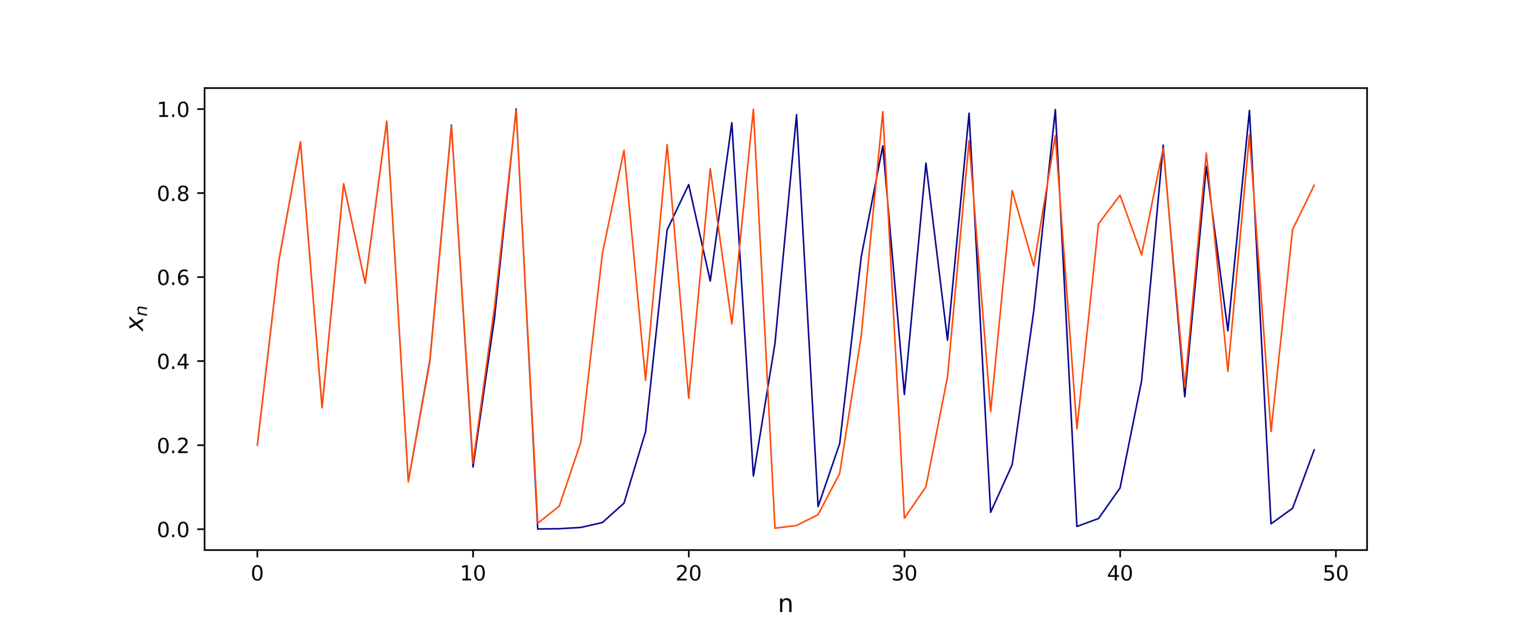
\includegraphics[scale=0.74]{Graphs/_logistic_sdic.eps}
        \centering
        \captionof{figure}{Figure generated for Logistic Map $x_{n+1}=rx_n(1-x_n)$ with $r=4$ to exhibit the presence of SDIC. Plotted are the values $x_n$ against time $n$ for the the first 50 step with initial values $x_0=0.2$ (blue) and $x_0=0.20001$ (red). Initially the two trajectories overlap, but they diverge completely at $n=12$ whereafter they follow distinct paths.}
        \label{fig:log_sdic}
      \end{figure}
  \ednote{B: Caption and figure adjusted}
  % For an intuitive sense of the fact that the LM exhibits SDIC, consider again the definition and substitute specific values. Let $\delta=0.05$ and for purposes of illustration consider the value $u=0.4$. The green band in~\ref{fig:log_sdic} shades the region $[u-\delta, u+\delta]$ and we can see that regardless the value $v$  and in every neighborhood of $u \in U$ there exists a $v\in{U}$ and an integer $N:=N{(u,v)}\in\mathbb{Z}$ such that $d(T^Nu,T^Nv)>\delta$
  % specific point, say $u=0.4$. Draw a green neighbourhood $[0.35,0.45]$ of diameters $\delta=0.02$ around the point. It is easy to see that every neighbourhood around $u=0.4$ will contain some $v_1, v_2\in[0,1]$ and natural number $N_1, N_2 \in\mathbb{N}$ respectively s.t. the distance $d(T^Nu_1,T^Nv)>\delta=0.05$ . 
\end{Example}


\begin{Example} \rm
  A second example pertains to a simple physical system called the double pendulum - a pendulum with another pendulum attached to its head given an initial position and angular velocity.  

  Below are two figures denoting trajectories of a double pendulum's second head after some elapsed time. Depicted are three pendulum heads with equal angular velocity but differing slightly in initial position. As can be seen below, the trajectories diverge very quickly to become completely different. We discuss the double pendulum in greater detail in a later chapter (\ref{ch5}), but we mention the example here to provide a numerical example of a practical system exhibiting SDIC.

\begin{figure}[ht]
  \centering
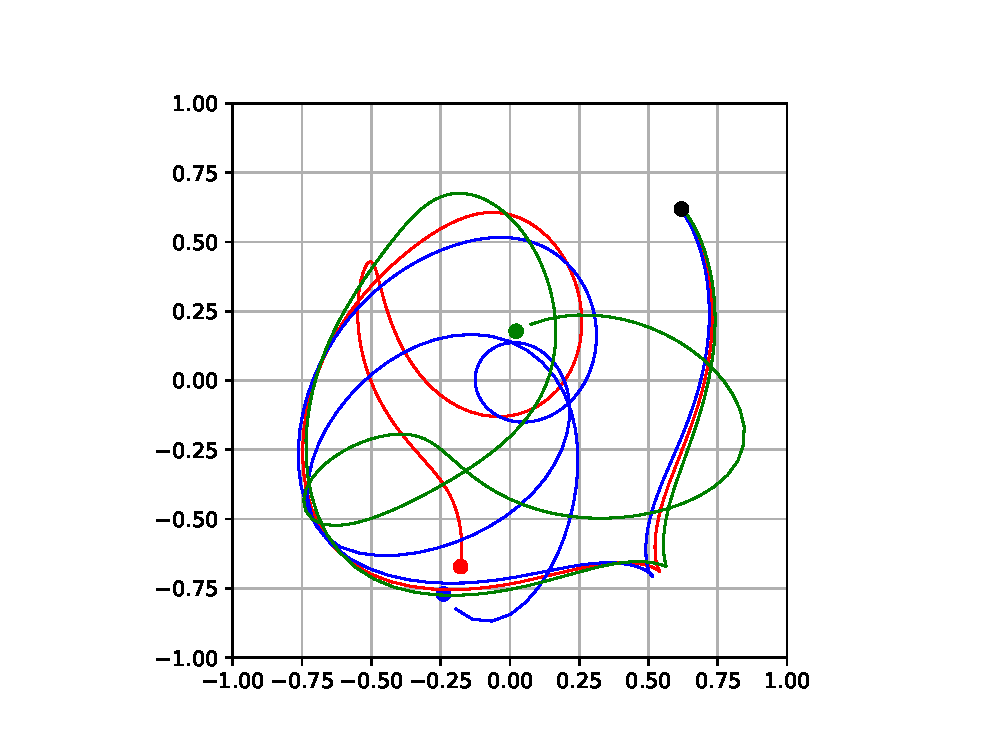
\includegraphics[scale=0.8]{Graphs/_dp_sdic.eps}
    \captionof{figure}{Three double pendulum heads with equal angular velocity and initial angles differing by 0,025 radians}\label{fig:dp_sdic}
  \end{figure}

\end{Example}


The second part in Devaney's definition of chaos concerns topological transitivity.

\begin{Definition}
  [\bf {Topologically Transitive}]\label{Dfn_TopolTrans}\rm
	A dynamical system $F: U \to U$ is topologically transitive if for any pair of nonempty open sets $E_1$ and $E_2$ there exists a $n\in\mathbb{N}$ such that $T^n(E_1) \cap E_2 \not= \emptyset$. 
\end{Definition}

Topological transitivity implies that iterates of an open set of initial conditions get mixed up with other open sets. On a compact metric space, one may show that topological transitivity also implies the existence of a point whose forward iterates are dense \cite{de2013elements}; or in other words, the orbit going through this point will be dense in the compact metric space. 
In fact, it is topologically more likely that the choice of an arbitrary point will be one whose iterates are almost dense. 

\begin{Definition}
  [\bf {Meager Set}]\label{Dfn_Meager Set}\rm
A subset of a topological space $U$ is said to be a meager set if it can be written as a countable union of sets of with empty interior. The complement of the a meager set is set to be a residual set.
\end{Definition}

To be more precise (see \cite{de2013elements}), for a discrete-time dynamical system on a compact space, the set of points with dense iterates are residual, and they are typical or likely to be observed in practice. In this project, when data is observed from a topologically transitive system, we assume it arises from a dense orbit.

We may now define the notion of Chaos as formulated by Devaney\cite{devaney2018introduction}.
\begin{Definition}
  [\bf {Devaney's Chaos}]\label{Dfn_ChaosDec}\rm
	A dynamical system $T: U \to U$ is said to exhibit chaos in the sense of Devaney if it satisfies the three properties:
	\vspace{-5mm}
  \begin{enumerate}
		\item $T$ has SDIC.
		\item $T$ is topologically transitive.
		\item The set of periodic points of $T$ are dense in $U$. 
	\end{enumerate}
\end{Definition}




\begin{Example} \rm
  The standard tent map $Tu=1-|2u-1|$ defined on $[0,1]$ is a well-known example of a dynamical system satisfying these three properties. 

  We now reason as to why this is true. The graph of the map $T$ is piecewise linear with two straight lines, one connecting the points $(0,0)$ and $(\frac{1}{2},1)$ and the other connecting $(\frac{1}{2},1)$ with $(1,0)$. They form a so-called tent with base centered at $u=1/2$. The graph of the map $T^2$ comprises two symmetric tents with their base centered at $1/4$ and $3/4$. See Figure \ref{fig:T2tentmap}

  \begin{figure}[ht]
    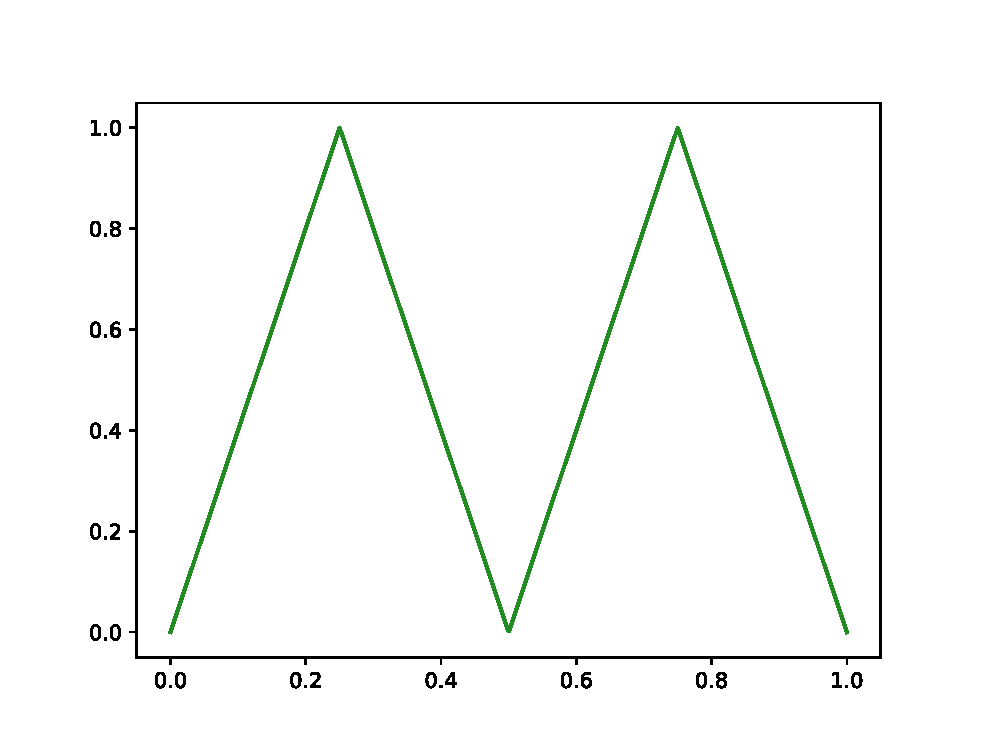
\includegraphics[scale=0.6]{Graphs/_tentmap_2.eps}
        \centering
        \captionof{figure}{Graph of the $T^2$ map with bases at $x=0$, $x=\frac{1}{2}$ and $x=1$ respectively.}\label{fig:T2tentmap}
  \end{figure}
  
  In general, the graph of  $T^k$ contains $2^{k-1}$ tents.
  Given any point $u$ and an open neighborhood $W \subset[0,1]$ of $u$, we can find $k\in\mathbb{Z}$ large enough so that $T^k(W) = [0,1]$ because we can accommodate a tent whose base is contained in $W$. % \ednote{B: This last phrase doesn't make sense to me. M: The number of tents grow with $k$ and hence this is obvious; I explained in one of our meetings. Does it make sense?} 
  This implies the existence of two points $w_1$ and $w_2$ in $W$ so that $d(T^kw_1,T^kw_2)= 1$, and by the triangle inequality  at least one of the inequalities $d(T^ku,T^kw_1)> \delta$ or $d(T^ku,T^kw_2)> \delta$ hold when $\delta\in (0,\frac{1}{2})$.  So $T$ has sensitive dependence on initial conditions.
  
  Next, let $W_1$ and $W_2$ be two nonempty open sets. Given any open set $W_1$, we can find a $k\in\mathbb{N}$ large enough so that $T^k(W_1) = [0,1]$ because we can accommodate a tent with base contained in $W$. So $T^k(W_1) \cap W_2 \not=\emptyset$, and thus $T$ has topological transitivity.
  
  Finally, for every open interval $(a,b)$, the graph of $T^k$ intersects the graph of the identity map on $[0,1]$. This follows from the fact established above that there exists a $k\in\mathbb{N}$ such that $T^k(a,b) = [0,1]$.If the intersection point has coordinates of the form $(p,p)$, the point $p$ is then a fixed point of $T^k$ and therefore also a periodic point of $T$. Since we have found a periodic point in the interval $W$,  the set of periodic points are dense in $T$.
  This follows because any fixed point of $T^k$ is also a periodic point, and we have found this in an arbitrary interval.


\end{Example}




\section{Conjugacy}

We now turn our attention to the subject of conjugacy that describes when two dynamical systems are equivalent dynamically. 

To show topological similarity (or sameness) between two metric or topological spaces, one needs to establish a homeomorphism between the two spaces. 
However, in the study of dynamical systems defined on two spaces, establishing a homeomorphism does not indicate that the systems are dynamically related in any way.
For instance, the maps $Tu=u^2$ and $Tu=1-|2u-1|$ defined on $[0,1]$ have totally different behaviour. 
Therefore, to find dynamically similar systems, one must establish a dynamical equivalence that we illustrate in a simple commutativity diagram below~\ref{eqn_conjugacy}.

% Giving errors
\begin{equation}  \label{eqn_conjugacy}
%    \[ 
    \psset{arrows=->, arrowinset=0.25, linewidth=0.6pt, nodesep=3pt, labelsep=2pt, rowsep=0.7cm, colsep = 1.1cm, shortput =tablr}
 \everypsbox{\scriptstyle}
 \begin{psmatrix}
U & U\\%
V & V.
 %%%
%  \ncline{1,1}{1,2}^{T} 
%  \ncline{1,1}{2,1} <{\phi}
%   \ncline{2,1}{2,2}^{S}
%  \ncline{1,2}{2,2} > {\phi}
 \end{psmatrix}
% \]
\end{equation} 

%Composite functions
To understand the diagram, we note that if we travel "right and then down," the diagram instructs us to use $T$ (top arrow right) first, followed by $\phi$. (right arrow downwards). Consequently, the pathway amounts to finding $\phi(T(u))$. If we proceed "down and then right," the diagram instructs us to apply $\phi$ (left arrow downwards) first, and then apply $S$ (bottom arrow right). This then amounts to finding  $S(\phi(u))$. When the relationships in this diagram hold, we say $\phi(T(u))= S(\phi(u))$, and we formally denote it as $\phi \circ T=S\circ \phi$.

\begin{Definition}\rm  
[\bf {Conjugacy \& Semi-Conjugacy}]\label{Dfn_Conjugate}\rm
   Consider the dynamical systems $T:U\to{U}$, $S:V\to{V}$ and suppose the relationship $\phi \circ T=S\circ \phi$ holds. If $\phi:U\to{V}$ is a homeomorphism, then $S$ is said to be conjugate to $T$ and $\phi$ is called a conjugacy. If we relax the criterion on $\phi$ and merely require $\phi$ to be continuous and surjective where $\phi:U\to{V}$, then $\phi$ is a semi-conjugacy between $T$ and $S$ where T has domain $U$ and S has domain $V$; S is said to be semi-conjugate to T. 
\end{Definition} 

\ednote{B: Does defining explicitly the domain and codomain of $\phi$ make it clear enough?  M: Saying $\phi$ is then a semi-conjugacy between $T$ and $S$ could be ambiguous as it does not specify which system is on the top in the commutativity. So please edit accordingly.}
When $S$ is conjugate to $T$, the dynamics of the two systems are in some way `dynamically equivalent'. Specifically, they are in one-to-one correspondence with one another. However when $S$ is semi-conjugate to $T$ with $\phi:U\to{V}$ a many-to-one mapping, the dynamics on $V$ provide merely a coarse-grained description of the dynamics on $U$~\cite{de2013elements}. When $S$ is semi-conjugate to $T$, it is also common to call $S$ a \emph{factor of $T$}, or conversely that $T$ is an \emph{extension of $S$}. In essence, an extension (see, \cite{de2013elements}) is a more extensive system capturing all of the essential dynamics of its factor.

It is a very hard or nearly an impossible task to establish the existence of a conjugacy or a semi-conjugacy $\phi$ between two systems \cite{devaney2018introduction}. However, one can verify that a function $\phi$ satisfies the commutativity diagram \ref{eqn_conjugacy}.  

\begin{Example}\rm
  For example $\phi(x)=\sin\big(\frac{\pi}{2}x\big)^2$ is a conjugacy between two systems $Tu=1-|2u-1|$ and $Sv=4v(1-v)$  defined on $U=[0,1]$.  

  Indeed, $\phi:[0,1]\to[0,1]$ is a homeomorphism and by employing simple trigonometric identities, it is easily proved that $\phi$ satisfies~\ref{eqn_conjugacy}
  \[
    \begin{aligned}[t]
      (\phi\circ{T})u 
                &=\sin^{2}\Big(\frac{\pi}{2} - \frac{\pi}{2}|2u-1|\Big) = \sin^{2}(\pi{u})=\Big(2\sin(\frac{\pi}{2})\cos(\frac{\pi}{2})\Big)^{2}=4\sin^{2}(\frac{\pi}{2}u)\Big(1-\sin^{2}\frac{\pi}{2}u\Big) \\
                                    &=({S}\circ\phi)u.
    \end{aligned}
\]
And it follows that $\phi$ is a conjugacy between the two systems.
\end{Example}


By establishing that two systems are conjugate (semi-conjugate) to one another, we have also shown that one may choose to work with one system instead of the second and still be guaranteed to obtain information on the latter. It is instrumental during the process of forecasting the future evolution of dynamical systems. 

